\chapter{Results}
\label{ch:results}

\section{Main findings}
Give the results in the order of the questions in \cref{ch:intro}, one subsection each,
and say what each result means in the same paragraph. \Cref{fig:trend} shows a figure drawn
in \LaTeX{} from data, so no image file is needed; replace it with
\verb|\includegraphics| for your own.

\begin{figure}[ht]
  \centering
  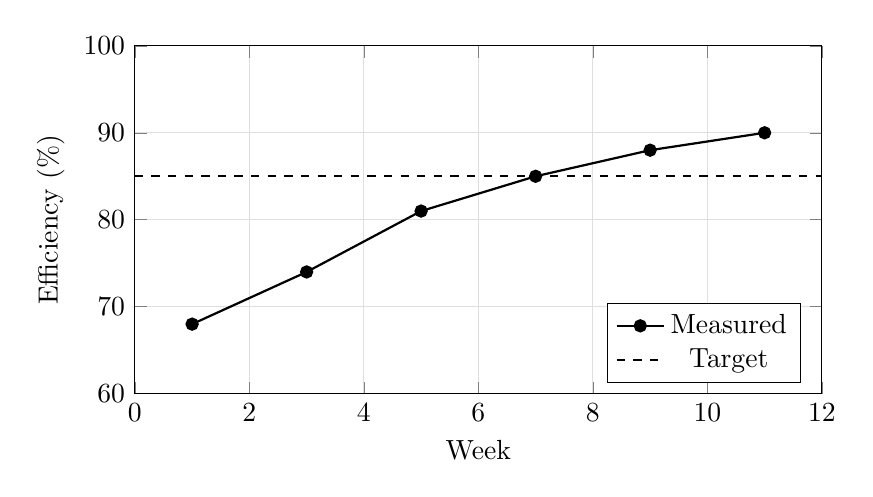
\begin{tikzpicture}
    \begin{axis}[width=0.85\textwidth, height=6cm, xlabel={Week}, ylabel={Efficiency (\%)},
                 xmin=0, xmax=12, ymin=60, ymax=100, grid=major, grid style={gray!25},
                 legend pos=south east]
      \addplot[thick, mark=*] coordinates {(1,68) (3,74) (5,81) (7,85) (9,88) (11,90)};
      \addplot[thick, dashed, domain=0:12] {85};
      \legend{Measured, Target}
    \end{axis}
  \end{tikzpicture}
  \caption{Efficiency $\eta$ from \cref{eq:efficiency} over the test period.}
  \label{fig:trend}
\end{figure}

\section{Comparison with the plan}
A table of planned against actual values lets the reader see at once what slipped.

\begin{table}[ht]
  \centering
  \caption{Planned and actual results.}
  \label{tab:plan}
  \begin{tabular}{@{}lrrl@{}}
    \toprule
    Item & Planned & Actual & Status \\
    \midrule
    Efficiency (\%) & 85 & 90 & Met \\
    Cost (k\texteuro) & 120 & 131 & Over budget \\
    Duration (weeks) & 12 & 11 & Met \\
    \bottomrule
  \end{tabular}
\end{table}
